%  !TeX  root  =  user_guide.tex

\section{SQL-Anywhere Plugin}\label{sec:sqlanywhere}

% when the revision of a section has been finalized, 
% comment out the following line:
% \updatedisclaimer

SQL Anywhere ist ein propriet�res relationales Datenbank-Managementsystem (RDBMS)
von Sybase. SQL Anywhere umfasst Unterst�tzung f�r r�umliche Daten einschlie�lich OGC, 
Shape-Dateien etc. sowie eingebaute Funktionen f�r den Export nach KML, GML und ins 
SVG-Format.

The \toolbtntwo{sqlanywhere}{SQL Anywhere} Plugin provides a native data provider 
added to QGIS under the GPL v3. The Plugin allows to connect to this SQL 
Anywhere. The \dialog{Add SQL Anywhere layer} dialog is similar in functionality 
to the dialogs for PostGIS and SpatiaLite.

F�r die \toolbtntwo{sqlanywhere}{SQL-Anywhere} Erweiterung wurde ein nativer 
Daten-Provider unter GPL v3 Lizens hinzugef�gt. Das Plugin erlaubt damit die Anbindung. 
Der \dialog{SQL-Anywhere Layer hinzuf�gen} Dialog ist in der Funktionalit�t �hnlich wie 
die Dialoge f�r PostGIS und SpatiaLite.

\begin{figure}[ht]
   \centering
   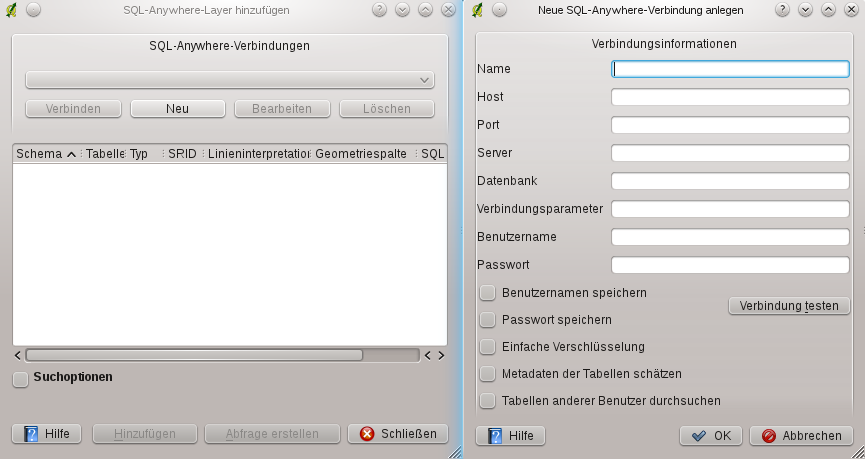
\includegraphics[clip=true, width=14cm]{sql_anywhere}
   \caption{SQL Anywhere Dialog \nixcaption}
   \label{fig:sqlanywhere}
\end{figure}

%% FIXME Needs an example, but the database is proprietary

\FloatBarrier
